
\documentclass[border=8pt, multi, tikz]{standalone}

\usepackage{import}
\subimport{./tex/}{init}

\usepackage{tikz}
\usetikzlibrary{quotes,arrows.meta}
\usetikzlibrary{positioning}
\usetikzlibrary{3d}

%Define the colors for different blocks
\definecolor{genericconvdark}{RGB}{255,193,98}
\definecolor{genericconv}{RGB}{252,210,147}
\definecolor{genericconvlight}{RGB}{253,226,184}

\definecolor{depthwisedark}{RGB}{94,238,118}
\definecolor{depthwise}{RGB}{131,249,151}
\definecolor{depthwiselight}{RGB}{171,255,185}

\definecolor{pointwisedark}{RGB}{255,193,98}
\definecolor{pointwise}{RGB}{252,210,147}
\definecolor{pointwiselight}{RGB}{253,226,184}

\definecolor{upconvdark}{RGB}{211, 104, 250}
\definecolor{upconv}{RGB}{215, 131, 246}
\definecolor{upconvlight}{RGB}{227, 163, 250}


% Connection style and colors for different operations
\definecolor{genericconvopcolor}{RGB}{253,226,184}
\newcommand{\genericconvop}{\tikz \draw[-Stealth,line width =1mm,draw=genericconvopcolor] (-0.3,0) -- ++(0.3,0);}

\definecolor{pointwiseopcolor}{RGB}{253,226,184}
\newcommand{\pointwiseop}{\tikz \draw[-Stealth,line width =1mm,draw=pointwiseopcolor] (-0.3,0) -- ++(0.3,0);}

\definecolor{depthwiseopcolor}{RGB}{253,226,184}
\newcommand{\depthwiseop}{\tikz \draw[-Stealth,line width =1mm,draw=depthwiseopcolor] (-0.3,0) -- ++(0.3,0);}

\definecolor{upconvopcolor}{RGB}{253,226,184}
\newcommand{\upconvop}{\tikz \draw[-Stealth,line width =1mm,draw=upconvopcolor] (-0.3,0) -- ++(0.3,0);}

\definecolor{depthwisepoolopcolor}{RGB}{253,226,184}
\newcommand{\depthwisepoolop}{\tikz \draw[-Stealth,line width =1mm,draw=depthwisepoolopcolor] (-0.3,0) -- ++(0.3,0);}

\definecolor{pointwisepoolopcolor}{RGB}{253,226,184}
\newcommand{\pointwisepoolop}{\tikz \draw[-Stealth,line width =1mm,draw=pointwisepoolopcolor] (-0.3,0) -- ++(0.3,0);}

\definecolor{convpoolopcolor}{RGB}{253,226,184}
\newcommand{\convpoolop}{\tikz \draw[-Stealth,line width =1mm,draw=convpoolopcolor] (-0.3,0) -- ++(0.3,0);}

\begin{document}
\begin{tikzpicture}

\tikzstyle{connection}=[ultra thick,every node/.style={sloped,allow upside down},opacity=0.7]
    

\node[canvas is zy plane at x=0] (in.jpeg) at (0,0,0)
{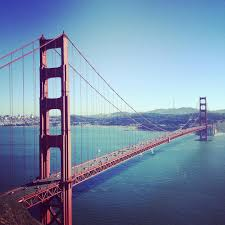
\includegraphics[width=128pt, height=128pt]{in.jpeg}};

\draw [connection] (0,0,0) -- node { \genericconvop} (3,0,0);

\pic[shift={(3,0,0)}] at (0,0,0)
	{ Box={ name=convolution1,caption= convolution1,xlabel={ { "", } }, ylabel = , zlabel = ,
	fillface=genericconvdark,
	fillfront=genericconvlight,
	fill=genericconv, height=15,width=3,depth=15 } };

\draw [connection] (convolution1-east) -- node { \pointwiseop} (6,0,0);

\pic[shift={(6,0,0)}] at (0,0,0)
	{ Box={ name=pointwise1,caption= pointwise1,xlabel={ { "", } }, ylabel = , zlabel = ,
	fillface=pointwisedark,
	fillfront=pointwiselight,
	fill=pointwise, height=15,width=3,depth=15 } };

\draw [connection] (pointwise1-east) -- node { \pointwiseop} (9,0,0);

\pic[shift={(9,0,0)}] at (0,0,0)
	{ Box={ name=pointwise2pool,caption= pointwise2pool,xlabel={ { "", } }, ylabel = , zlabel = ,
	fillface=pointwisedark,
	fillfront=pointwiselight,
	fill=pointwise, height=12,width=3,depth=12 } };

\draw [connection] (pointwise2pool-east) -- node { \depthwiseop} (12,0,0);

\pic[shift={(12,0,0)}] at (0,0,0)
	{ RightBandedBox={ name=depthwise1,caption= depthwise1,xlabel={ { "", } }, ylabel = , zlabel = ,
	fillface=depthwisedark,
	fillfront=depthwiselight,
	bandfill=depthwise,
	fill=depthwise, height=10,width=3,depth=10 } };

\draw [connection] (depthwise1-east) -- node { \depthwiseop} (15,0,0);

\pic[shift={(15,0,0)}] at (0,0,0)
	{ RightBandedBox={ name=depthwise1pool,caption= depthwise1pool,xlabel={ { "", } }, ylabel = , zlabel = ,
	fillface=depthwisedark,
	fillfront=depthwiselight,
	bandfill=depthwise,
	fill=depthwise, height=10,width=6,depth=10 } };

\draw [connection] (depthwise1pool-east) -- node { \pointwiseop} (18,0,0);

\pic[shift={(18,0,0)}] at (0,0,0)
	{ Box={ name=pointwise3,caption= pointwise3,xlabel={ { "", } }, ylabel = , zlabel = ,
	fillface=pointwisedark,
	fillfront=pointwiselight,
	fill=pointwise, height=8,width=6,depth=8 } };

\draw [connection] (pointwise3-east) -- node { \pointwiseop} (21,0,0);

\pic[shift={(21,0,0)}] at (0,0,0)
	{ Box={ name=pointwise4pool,caption= pointwise4pool,xlabel={ { "", } }, ylabel = , zlabel = ,
	fillface=pointwisedark,
	fillfront=pointwiselight,
	fill=pointwise, height=8,width=8,depth=8 } };

\draw [connection] (pointwise4pool-east) -- node { \upconvop} (24,0,0);

\pic[shift={(24,0,0)}] at (0,0,0)
	{ Box={ name=upconv1,caption= upconv1,xlabel={ { "", } }, ylabel = , zlabel = ,
	fillface=upconvdark,
	fillfront=upconvlight,
	fill=upconv, height=8,width=10,depth=8 } };

\draw [connection] (upconv1-east) -- node { \genericconvop} (27,0,0);

\pic[shift={(27,0,0)}] at (0,0,0)
	{ Box={ name=convolution2,caption= convolution2,xlabel={ { "", } }, ylabel = , zlabel = ,
	fillface=genericconvdark,
	fillfront=genericconvlight,
	fill=genericconv, height=12,width=6,depth=12 } };

\draw [connection] (convolution2-east) -- node { \upconvop} (30,0,0);

\pic[shift={(30,0,0)}] at (0,0,0)
	{ Box={ name=upconv2,caption= upconv2,xlabel={ { "", } }, ylabel = , zlabel = ,
	fillface=upconvdark,
	fillfront=upconvlight,
	fill=upconv, height=15,width=6,depth=15 } };

\draw [connection] (upconv2-east) -- node { \genericconvop} (33,0,0);

\pic[shift={(33,0,0)}] at (0,0,0)
	{ Box={ name=convolution3,caption= convolution3,xlabel={ { "", } }, ylabel = , zlabel = ,
	fillface=genericconvdark,
	fillfront=genericconvlight,
	fill=genericconv, height=18,width=3,depth=18 } };

\draw [connection] (convolution3-east) -- node { \upconvop} (36,0,0);

\pic[shift={(36,0,0)}] at (0,0,0)
	{ Box={ name=upconv3,caption= upconv3,xlabel={ { "", } }, ylabel = , zlabel = ,
	fillface=upconvdark,
	fillfront=upconvlight,
	fill=upconv, height=20,width=3,depth=20 } };

\draw [connection] (upconv3-east) -- node { \genericconvop} (39,0,0);

\node[canvas is zy plane at x=0] (out.jpeg) at (39,0,0)
{
\includegraphics[width=128pt, height=128pt]{out.jpeg}};

\draw [connection] (3,0,0) -- node { \depthwiseop} (3,0,15);

\draw [connection] (3,0,15) -- node { \depthwiseop} (8,0,15);

\pic[shift={(8,0,15)}] at (0,0,0)
	{ RightBandedBox={ name=residualdepth1,caption= residualdepth1,xlabel={ { "", } }, ylabel = , zlabel = ,
	fillface=depthwisedark,
	fillfront=depthwiselight,
	bandfill=depthwise,
	fill=depthwise, height=12,width=3,depth=12 } };

\draw [connection] (residualdepth1-east) -- node { \depthwiseop} (33,0,15);

\draw [connection] (33,0,15) -- node { \depthwiseop} (33,0,0);

\draw [connection] (9,0,0) -- node { \depthwiseop} (9,0,10);

\draw [connection] (9,0,10) -- node { \depthwiseop} (14,0,10);

\pic[shift={(14,0,10)}] at (0,0,0)
	{ RightBandedBox={ name=residualdepth1,caption= residualdepth1,xlabel={ { "", } }, ylabel = , zlabel = ,
	fillface=depthwisedark,
	fillfront=depthwiselight,
	bandfill=depthwise,
	fill=depthwise, height=10,width=3,depth=10 } };

\draw [connection] (residualdepth1-east) -- node { \depthwiseop} (27,0,10);

\draw [connection] (27,0,10) -- node { \depthwiseop} (27,0,0);

\draw [connection] (18,0,0) -- node { \depthwiseop} (18,0,6);

\draw [connection] (18,0,6) -- node { \depthwiseop} (21,0,6);

\pic[shift={(21,0,6)}] at (0,0,0)
	{ RightBandedBox={ name=residualdepth1,caption= residualdepth1,xlabel={ { "", } }, ylabel = , zlabel = ,
	fillface=depthwisedark,
	fillfront=depthwiselight,
	bandfill=depthwise,
	fill=depthwise, height=8,width=3,depth=8 } };

\draw [connection] (residualdepth1-east) -- node { \depthwiseop} (23,0,6);

\draw [connection] (23,0,6) -- node { \depthwiseop} (23,0,0);


\end{tikzpicture}
\end{document}
    